\documentclass{article}
\usepackage[T1]{fontenc}
\usepackage[utf8]{inputenc}
\usepackage[polish]{babel}
\usepackage{geometry}
\usepackage{hyperref} % klikalna bibliografia i spis treści
\usepackage{lmodern} % ładniejsze fonty
\usepackage{graphicx}
\usepackage{float}
\usepackage{indentfirst}
\usepackage{xurl}
\usepackage[backend=bibtex, style=numeric]{biblatex}
\addbibresource{references.bib}

\geometry{
    a4paper,
    left=3.5cm,
    right=3cm,
    top=3cm,
    bottom=3cm
}

\nocite{*}

\begin{document}

\begin{titlepage}
    \centering

    \vspace*{2cm}
    {\Large\bfseries UNIWERSYTET GDAŃSKI}\\[1.5em]
    {\large\bfseries WYDZIAŁ MATEMATYKI, FIZYKI I INFORMATYKI}

    \vfill

    {\large Bartłomiej Wnuk, Michał Witkowski, Wiktor Sieracki}\\
    {\large 285786, 278862, 285769}\\[4em]

    {Kierunek: Informatyka Praktyczna}\\[2.5em]

    \vfill

    {\huge\bfseries System informatyczny wspomagający wyszukiwanie i ocenę lokalizacji miejskich - Mapzilla}\\[6em]

    \vfill

    {\large Praca licencjacka}\\[1em]

    {napisana pod kierunkiem}\\[1.5em]

    dr. Adama Kostulaka, prof. UG \\[2em]

    \vfill

    {\large Gdańsk 2025}

    \vspace*{1cm}

\end{titlepage}

\tableofcontents
\newpage

\section{Opis problemu}

Patrząc na ciągle rozwijający się rynek nieruchomości, konsumenci mogą mieć problem z wyborem odpowiadającego im miejsca do zamieszkania. Brak dostępu do kluczowych zasobów w mieście powoduje u ludzi wybieranie mniej płatnych prac oraz pogłębia różnice społeczne. Dzieci, które mają gorszy dostęp do szkoły, często gorzej radzą sobie w nauce oraz mają mniej czasu na pogłębianie swoich zainteresowań.
\\

\noindent
\textbf{Czym jest miasto 15 minut?}  


Miasto 15 minut to koncepcja urbanistyczna, w której mieszkańcy mają dostęp do najważniejszych udogodnień w zasięgu 15 minut pieszo. Do udogodnień zalicza się szkoły, sklepy spożywcze, apteki, przychodnie oraz miejsca rekreacji.

\begin{figure}[H]
    \centering
    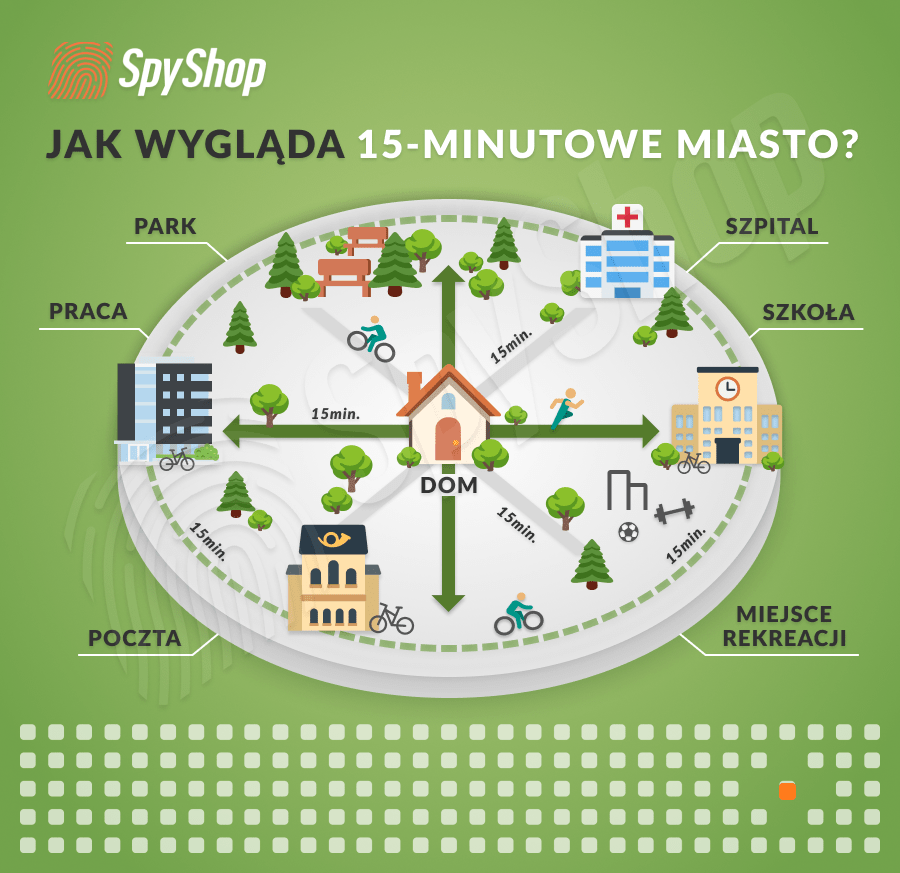
\includegraphics[width=0.75\linewidth]{miasto15minut.png}
    \caption{Miasto 15-minut \cite{miasto15minut}}
    \label{fig:enter-label}
\end{figure}

\noindent
\textbf{Jak osiągnąć status miasta 15 minut?}

Żeby dobrze rozplanować gdzie zbudować nowe miejsca codziennego użytku należy śledzić położenie zbudowanych już struktur. W aplikacji można łatwo zauważyć miejsca, w których jest gorszy dostęp do sklepów. Czy w pobliżu znajduje się szkoła.  

Dzięki aplikacji władze miasta mogą monitorować takie krytyczne miejsca i na jej podstawie rozplanowywać inwestycje na przyszłe lata. Należy zauważyć, że sprawna komunikacja miejska nie jest sposobem na zostanie miastem 15 minut. Trzeba jednak pójść o krok dalej i skupić się na inteligentnym rozmieszczeniu każdej budowli. Warto też trzymać się zasad takich jak budowanie większej ilości przestrzeni dla ludzi niż dla samochodów.
\\

\noindent
\textbf{Miasta, które są miastami 15 minut}

Przykładowe miasta spełniające wymagania miasta 15 minut to:
\begin{itemize}
    \item Barcelona - jest prekursorem jeżeli chodzi o rozwiązania miasta 15 minut. Jako miasto liczące ponad półtora miliona mieszkańców, osiągnęło miano miasta 15 minut dzięki swojej wielkiej gęstości zaludnienia oraz specyficznej zabudowie bloków widocznej na Rysunku 2. Na terenie miasta i okolic (Sant Adrià de Besòs, L’Hospitalet de Llobregat, Esplugues de Llobregat y Cornellà de Llobregat) obowiązuje tzw. Strefa Niskiej Emisji (Zona de Bajas Emisiones – ZBE). Oznacza to ograniczenie wjazdu na teren ZBE dla pojazdów osobowych niespełniających wymogów dot. emisji spalin od poniedziałku do piątku w godzinach od 7 do 20. \cite{gov}
    \begin{figure}[H]
        \centering
        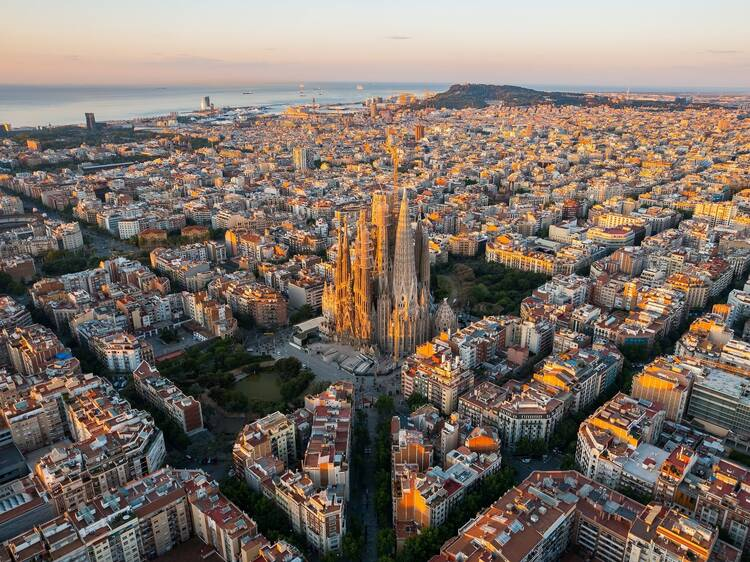
\includegraphics[width=1\linewidth]{barcelona.png}
        \caption{Barcelona \cite{barcelona}}
        \label{fig:enter-label}
    \end{figure}
    \item Melbourne - wspiera lokalne firmy,
    \item Portland - buduje mieszkania komunalne w bogatych dzielnicach,
    \item Paryż - dba o rozbudowe zielonych terenów przyszkolnych.
\end{itemize}
\\

\noindent
\textbf{Zalety miasta 15 minut}

W opisie problemu przedstawiono niektóre wady braku dostępu do kluczowych struktur w mieście. Z kolei do zalet należą:

\begin{itemize}
    \item mniejsze zanieczyszczenie miasta spalinami,
    \item poprawa jakości życia mieszkańców,
    \item oszczędność czasu przeznaczanego na dojazdy,
    \item zwiększenie integracji społecznej,
    \item większa aktywność fizyczna mieszkańców.
\end{itemize}

\section{Porównanie dostępnych rozwiązań}

\textbf{Mapy Google} — pozwalają zobaczyć znajdujące się dookoła udogodnienia, lecz nie skupiają się na ich kompleksowej analizie i nie przedstawiają ich w dogodny sposób dla użytkownika planującego wybór miejsca zamieszkania.

\textbf{15-min city} — (https://app.developer.here.com/15-min-city-map/) mała aplikacja działająca tylko na terenie stanów zjednoczonych. Brak możliwości wyboru pożądanych miejsc.

\section{Możliwości zastosowania praktycznego}

\begin{itemize}
    \item \textbf{Dla mieszkańców} — pomoc w wyborze odpowiedniego miejsca do zamieszkania.
    \item \textbf{Dla deweloperów} — planowanie inwestycji mieszkaniowych w najlepszych lokalizacjach, poprawiających komfort życia lokatorów.
    \item \textbf{Dla władz miasta} — rozwój infrastruktury społecznej oraz planowanie przestrzenne zgodne z potrzebami mieszkańców.
\end{itemize}


Poniżej widać strukture komunikacji poszczególnych serwisów w naszej aplikacji.

\begin{figure}[H]
    \centering
    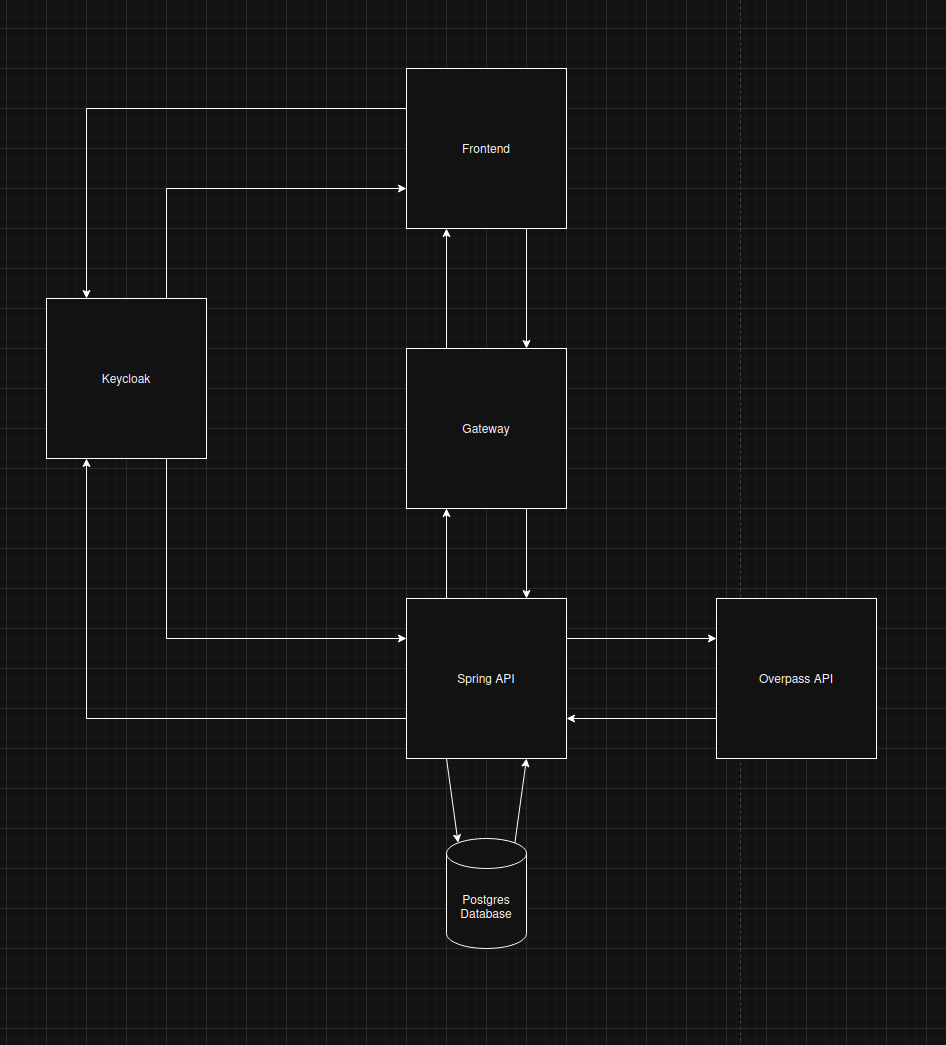
\includegraphics[width=1\linewidth]{struktura.png}
    \caption{Struktura projektu}
    \label{fig:struktura}
\end{figure}

Diagram autentykacji użytkownika.

\begin{figure}[H]
    \centering
    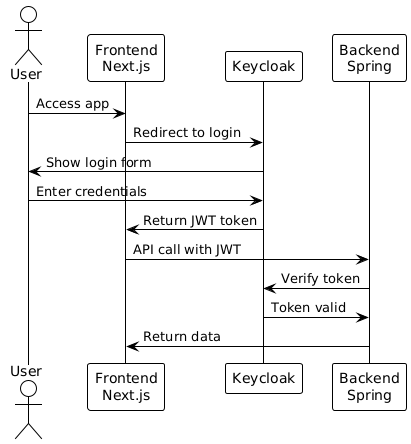
\includegraphics[width=1\linewidth]{autentykacja.png}
    \caption{Autentykacja}
    \label{fig:enter-label}
\end{figure}

Przypadki użycia aplikacji.

\begin{figure}[H]
    \centering
    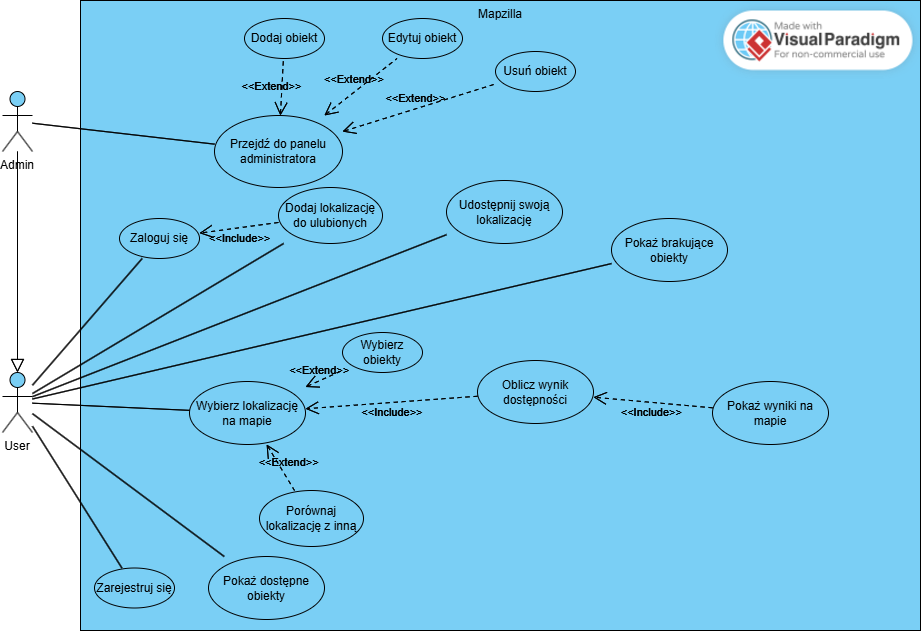
\includegraphics[width=1\linewidth]{przypadki_uzycia.png}
    \caption{Przypadki użycia}
    \label{fig:porownywanie}
\end{figure}

Diagram Klas.

\begin{figure}[H]
    \centering
        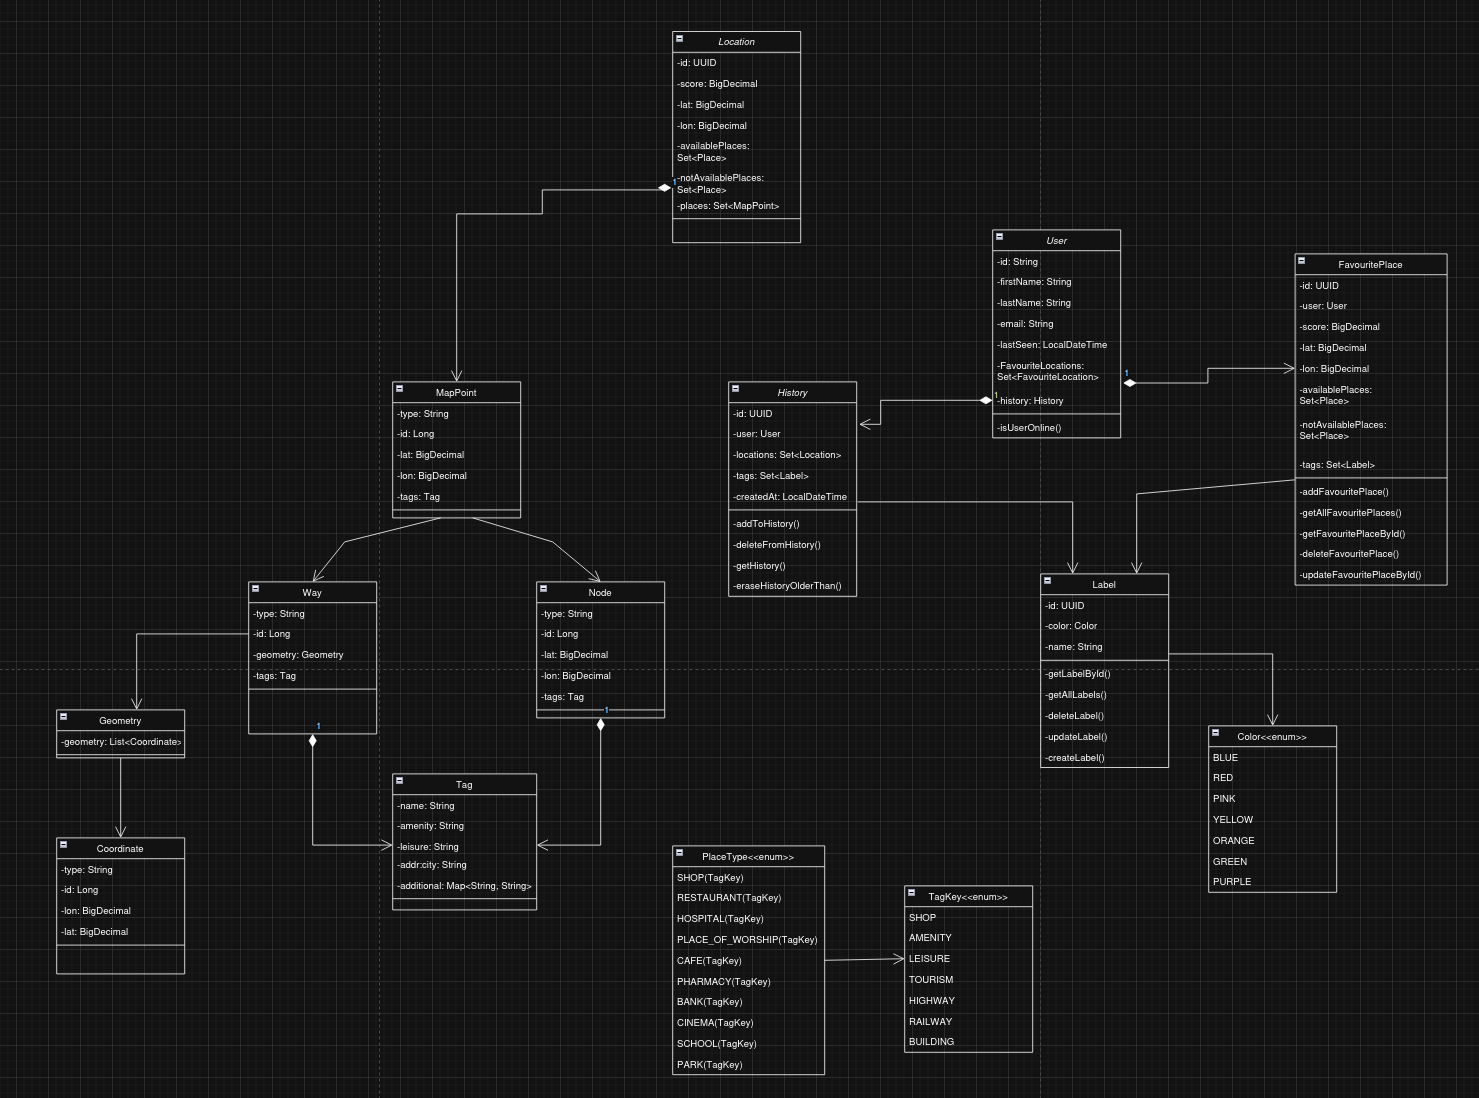
\includegraphics[width=1\linewidth]{diagram_klas.png}
    \caption{Diagram Klas}
    \label{fig:diagram klas}
\end{figure}

\section{Wymagania}

\noindent\textbf{Funkcjonalne} \\

Mapa w Aplikacji znajduje obiekty w całej Polsce. \\

Dostępne jest wiele atrakcji do wyboru z listy. \\

Możliwa jest rejestracja użytkownika. \\

Możliwe jest logowanie użytkownika. \\

\noindent\textbf{Niefunkcjonalne} \\

Mapa działa płynnie. \\

Użytkownik zostaje wylogowany po 5 minutach nieaktywności. \\

Dane użytkowników są bezpiecznie przechowywane. \\

\section{Użytkowanie Aplikacji}

\noindent\textbf{Rejestracja Użytkownika}

Aby zarejestrować się w aplikacji, należy podać swoje dane osobowe oraz adres e-mail. Odbywa się to poprzez Keycloak, który jest zintegrowany z aplikacją. Dzięki temu, że użyliśmy sprawdzonego pośrednika do zarządzania użytkownikami, zapewniamy większe bezpieczeństwo ich danych.

\begin{figure}[H]
    \centering
    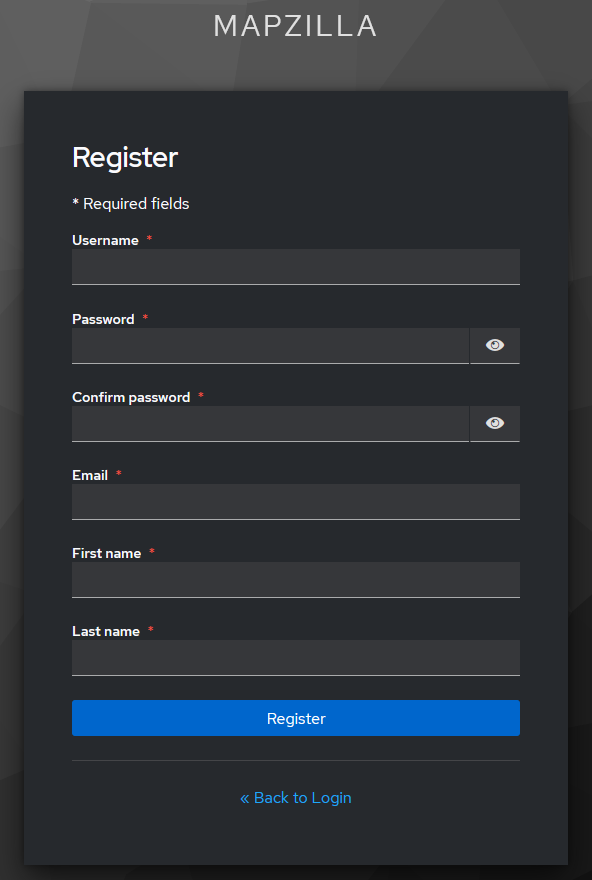
\includegraphics[width=0.5\linewidth]{rejestracja.png}
    \caption{Rejestracja}
    \label{fig:rejestracja}
\end{figure}

\noindent\textbf{Logowanie Użytkownika}

Aby zalogować się do aplikacji, należy podać swoją nazwę użytkownika oraz hasło. Po zalogowaniu użytkownik zostaje przekierowany do strony głównej aplikacji. Stamtąd może dodawać do ulubionych lokalizacje.

\begin{figure}[H]
    \centering
    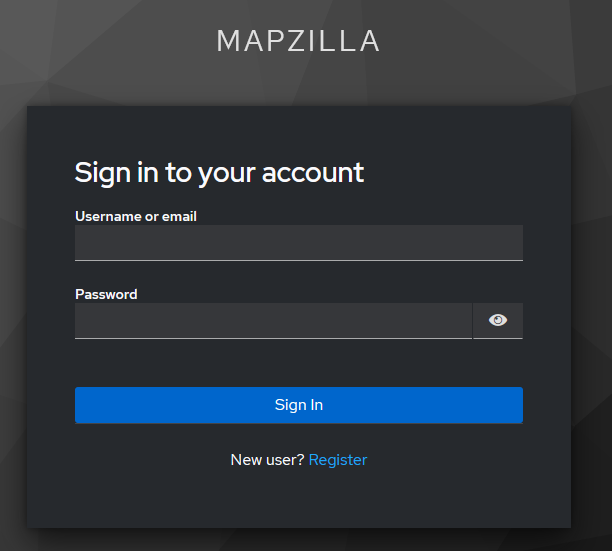
\includegraphics[width=0.5\linewidth]{logowanie.png}
    \caption{Logowanie}
    \label{fig:logowanie}
\end{figure}

\noindent\textbf{Wyszukiwanie miejsc po nazwie}

Dzięki wyszukiwarce użytkownik może znaleźć interesujące go miejsca. Wystarczy wpisać nazwę miejsca miasta lub ulicy, a aplikacja przeniesie nas do wybranego miejsca, z którego możemy dalej szukać interesujących nas obiektów.

\begin{figure}[H]
    \centering
    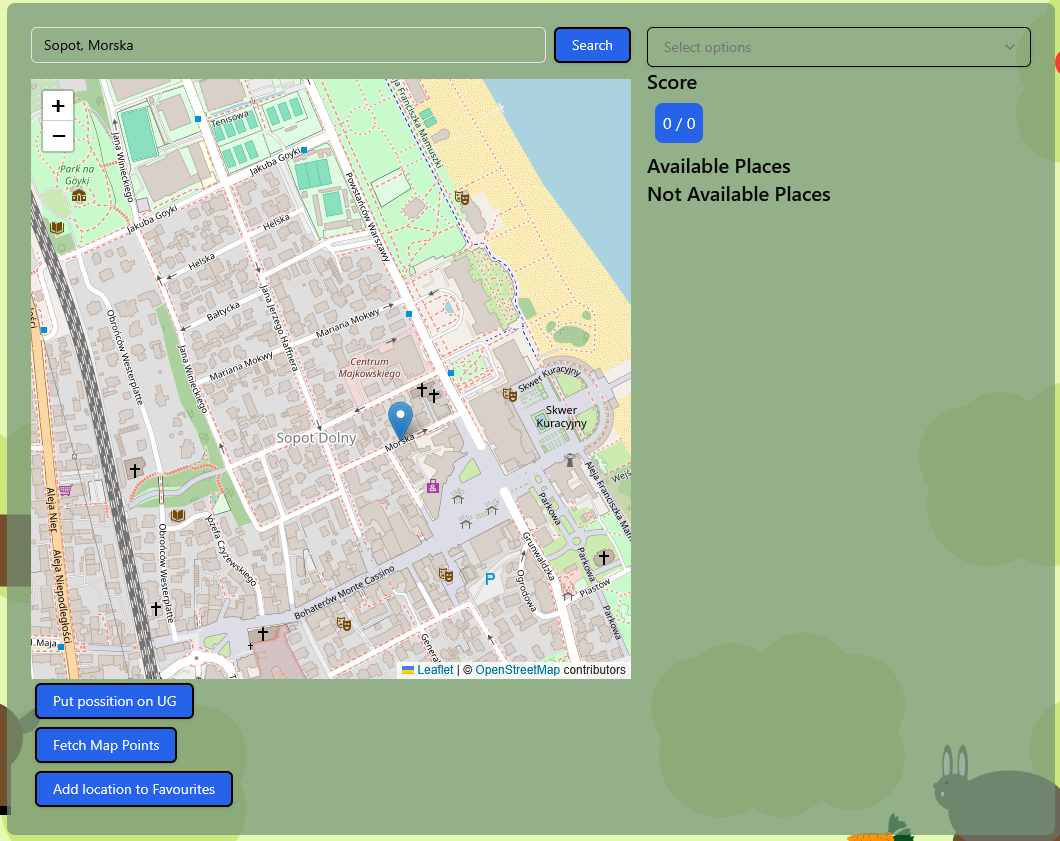
\includegraphics[width=1\linewidth]{wyszukiwarka.png}
    \caption{Wyszukiwanie miejsca}
    \label{fig:wyszukiwanie}
\end{figure}

\noindent\textbf{Mapa z Lokalizacjami}

Głównym działaniem naszej aplikacji jest mapa, która pozwala na przeglądanie oraz wyszukiwanie interesujących nas lokalizacji. Użytkownik może wybrać interesujące go miejsca i wyszukać ich w okolicy.

\begin{figure}[H]
    \centering
    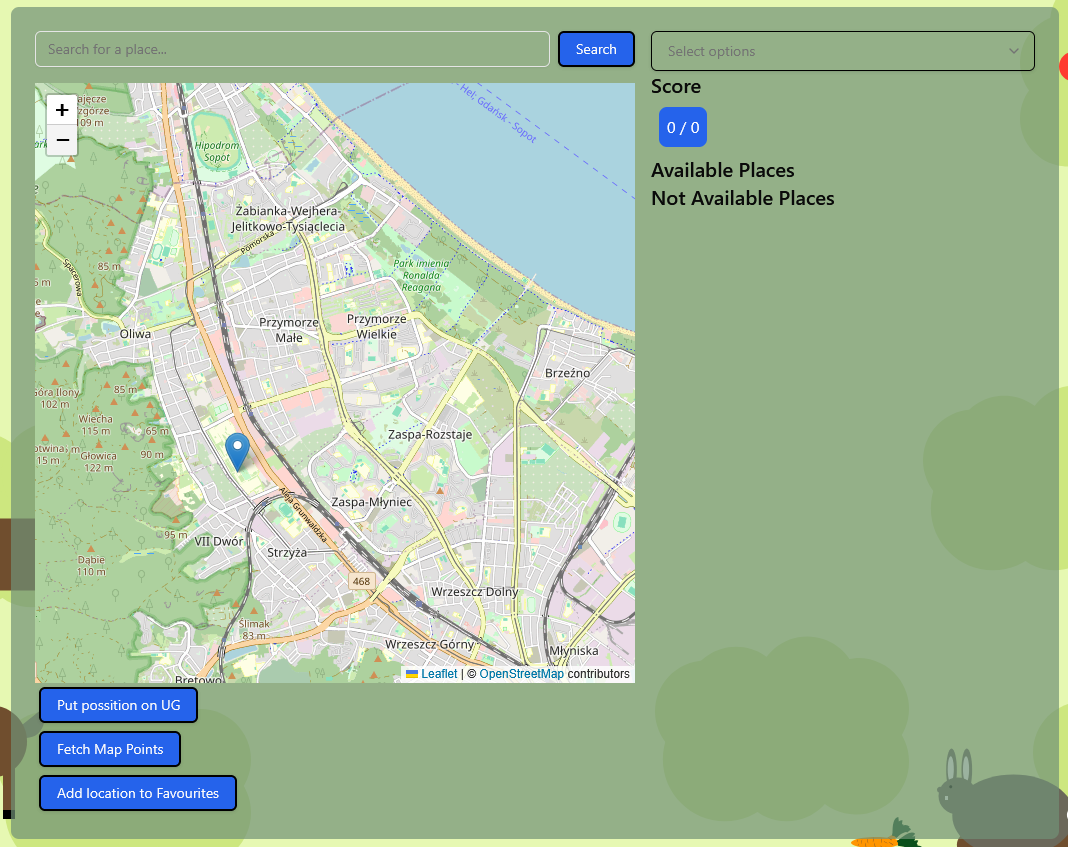
\includegraphics[width=1\linewidth]{mapa.png}
    \caption{Mapa}
    \label{fig:mapa}
\end{figure}

\noindent\textbf{Ulubione miejsca}

Po kliknięciu w nazwę użytkownika w prawym górnym rogu, możemy przejść do zakładki ulubione miejsca. Można tam zauważyć listę ulubionych miejsc, które użytkownik dodał do swojego konta. Każde miejsce ma opisany wynik, koordynaty oraz dostępne i niedostępne tam udogodnienia.

\begin{figure}[H]
    \centering
    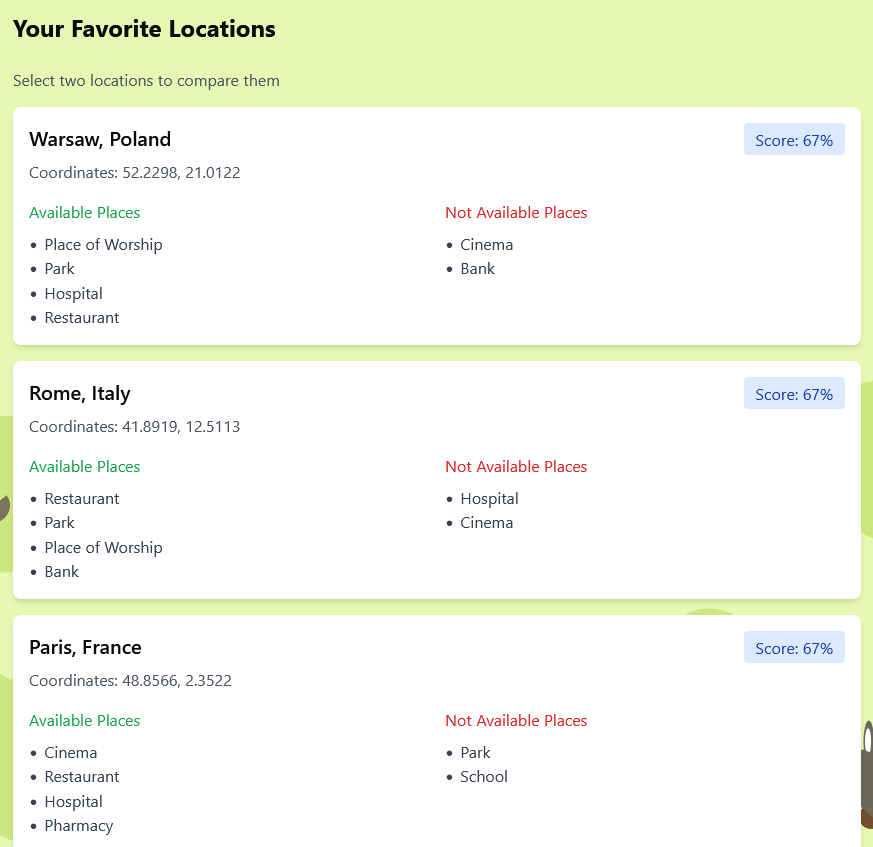
\includegraphics[width=1\linewidth]{ulubione.png}
    \caption{Ulubione}
    \label{fig:ulubione}
\end{figure}

\noindent\textbf{Ulubione miejsca}

Klikając na dwa interesujące nas ulubione miejsca możemy je ze sobą porównać.

\begin{figure}[H]
    \centering
    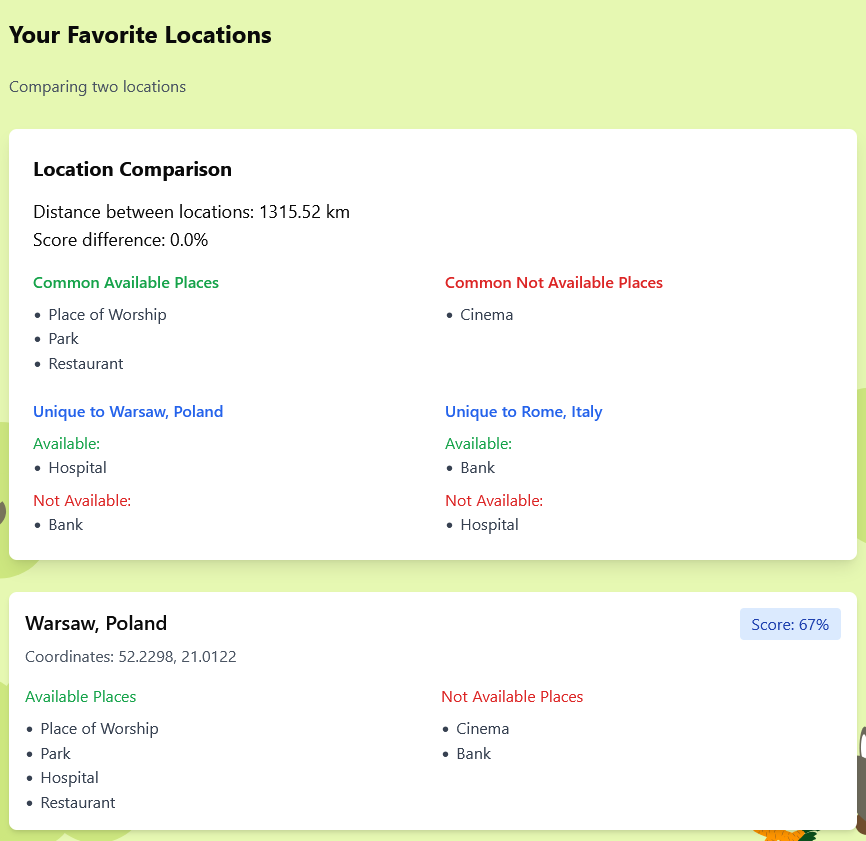
\includegraphics[width=1\linewidth]{porownywanie.png}
    \caption{Porównywanie ulubionych miejsc}
    \label{fig:porownywanie}
\end{figure}

\section{Wzorce projektowe}

Tworząc aplikację korzystaliśmy z wzorca RESTFul, który służy do wydajnego posługiwania się i korzystania z HTTP oraz jego standardowych metod takich jak GET, POST, PUT, DELETE, PATCH. Wykorzystujemy wersjonowanie zawarte w adresie oraz statusy HTTP. Z innych dobrych praktyk, w adresach posługujemy się liczbą \texttt{/favourite-places}.

Standardową praktyką w Spring Boot, z której korzystamy, jest używanie Dependency Injection, czyli wstrzykiwania zależności do obiektów, co pozwala na luźne powiązanie komponentów, które wspiera modularność, ułatwia testowanie oraz sprawia, że projekt jest łatwiejszy w utrzymaniu. Wzorzec Strategy pozwala nam na wybór odpowiednich algorytmów służących do serializacji danych. Spring Boot sam w sobie korzysta z wzorców projektowych takich jak Singleton czy Factory. Oba są powiązane z bean'ami. Pierwszy z nich odpowiada za to, że tworzona i zarządzana jest tylko jedna instancja danej klasy. Ułatwia to zarządzanie cyklem ich życia oraz zarządzaniem zasobami. Natomiast drugi odpowiada za samo tworzenie bean'ów na podstawie definicji konfiguracyjnych.

Wzorzec Gateway to bardzo użyteczny i ważny wzorzec projektowy w kontekście zabezpieczeń aplikacji. Służy on do enkapsulacji dostępu do zewnętrznego systemu lub usługi. Wprowadza on łatwe rozwijanie aplikacji w stronę architektury opartej na mikroserwisach, gdzie pełni rolę pojedynczego punktu wejścia dla wszystkich żądań, a następnie przekierowywania ich w odpowiednie miejsca. Może on też pełnić rolę agregowania odpowiedzi, uwierzytelniać, autoryzować oraz logować do aplikacji. W kontekście serwera działającego jako monolit, serwis będący jako Gateway pełni rolę izolowania strony serwera przed niechcianym wejściem, natomiast monolit posiadający całą logikę biznesową aplikacji staje się kolejną usługą.

Tworząc stronę serwera, korzystamy również z wzorca 3-Tier Architecture, który dzieli całą aplikację na trzy różne poziomy: poziom prezentacji, poziom aplikacji oraz poziom danych. Takie podejście pomaga odseparować od siebie moduły i pozwala na większe bezpieczeństwo, dzięki temu, że poziom prezentacji oraz poziom danych nie mogą się ze sobą bezpośrednio kontaktować, co zapobiega atakom hakerskim takim jak SQL Injection. Wpływa to też na niezawodność całego projektu, gdyż błąd na jednym poziomie nie zawsze oznacza błąd na drugim poziomie. Pozwala też na większą skalowalność, każdy z poziomów może skalować się niezależnie od reszty. Podejście to też wpływa na szybkość rozwoju aplikacji, która może być rozwijana na każdym poziomie przez oddzielne zespoły programistów. Na samym poziomie aplikacji korzystamy z podejścia 3-Layer Architecturem, który dzieli aplikację na trzy niezależne warstwy: warstwę prezentacji, czyli kontrolery, warstwę logiki biznesowej czyli serwisy oraz warstwę danych czyli repozytoria.

\section{Użyte technologie}

Po stronie serwera posiadamy API napisane w framework javy, Spring Framework. Dokładniej, korzystamy z nakładki Spring Boot, która ma za zadanie uprościć proces tworzenia projektu zawierając w sobie serwery takie jak Tomcat, automatycznie konfiguruje aplikację.
\\

Oprócz tego nasz projekt korzysta z bibliotek takich jak Lombok. Jest to biblioteka, która dostarcza adnotacje, które w sposób znaczący zmniejszają ilość potrzebnego kodu i sprawiają, że sama aplikacja jest przejrzysta i bardziej czytelna. Innym narzędziem, z którego korzystamy jest OpenApi, które dostarcza Swagger, czyli instrument do automatycznego generowania dokumentacji na podstawie kontrolerów, jakie nasza aplikacja posiada.
\\

Do mapowania obiektowo-relacyjnego wykorzystujemy framework Hibernate. Pozwala on na mapowanie obiektów w języku Java na tabele w bazie danych i posługiwanie się operacjami bazodanowymi używając wysokopoziomowego API, dzięki czemu nie musimy pisać niskopoziomowego kodu SQL. 
\\

Informacje o użytkownikach oraz logikę rejestracji i logowania użytkowników rozwiązaliśmy za pomocą serwisu Keycloak. Dzięki niemu możemy nadawać użytkownikom odpowiednie role oraz weryfikować ich maile.
\\

Nasza baza danych znajduje się w PostgreSQL, przechowujemy tam informacje o lokalizacjach oraz ich relacje z użykownikami.
\\

Do napisania warstwy widocznej w przeglądarce użyliśmy biblioteki React. Przy pomocy framework'a Next.js dzielimy pliki na komponenty klienta i serwera. Do budowania responsywnych interfejsów użytkownika użyliśmy frameworka Tailwind CSS. Używamy też gotowych komponentów UI z biblioteki Shadcn.
\\

Do autoryzacji użytkowników w przeglądarce używamy biblioteki Next-Auth. Pozwala na odszyfrowanie tokenów JWT i pozyskanie danych z Keycloak. 
\\

Dzięki narzędziu Docker możemy sprawnie konteneryzować nasze serwisy, co pozwala na lepszą kontrolę wersji oraz ułatwia późniejszą skalowalność aplikacji.
\\


\section{Testowanie Aplikacji}

Testowanie aplikacji Mapzilla stanowiło istotny element procesu wytwarzania oprogramowania. Celem testów było sprawdzenie funkcjonalności aplikacji, walidacji danych oraz obsługi błędów. Zastosowano dwa rodzaje testowania: 

\begin{itemize}
    \item \textbf{Testy jednostkowe} - automatyczne testy napisane w języku Java z wykorzystaniem biblioteki JUnit oraz narzędzi takich jak Mockito i Spring Boot Test. Przetestowano logikę odpowiedzialną za obsługę żądań związanych z ulubionymi lokalizacjami użytkownika.
    \item \textbf{Testy manualne} - testy wykonywane ręcznie z użyciem narzędzia Postman. Polegały one na wysyłaniu żądań HTTP do enpointów REST API w działającej aplikacji. Sprawdzono poprawność odpowiedzi serwera, walidację danych wejściowych, oraz działanie mechanizmu autoryzacji z wykorzystaniem tokenów JWT.
\end{itemize}

\noindent\textbf{Scenariusze testowe} 

W ramach testowania aplikacji przygotowano zestaw scenariuszy testowych, które miały na celu zweryfikowanie poprawności działania najważniejszych funkcjonalności systemu. Scenariusze te objęły zarówno pozytywne, jak i negatywne przypadki użycia. Poniżej przedstawiono listę metod testowych wraz z ich krótkim opisem:

\begin{itemize}
    \item \textbf{createLocation\_ReturnCreated} - sprawdza, czy po przesłaniu poprawnych danych lokalizacji system poprawnie tworzy nowy wpis.
    \item \textbf{createLocation\_ReturnCreated\_CheckResponse} - sprawdza, czy po przesłaniu poprawnych danych lokalizacji system zwraca poprawne dane, takie jak wartość pola \texttt{score}
    \item \textbf{createLocation\_ReturnBadRequest\_Score} - testuje reakcję systemu na przesłanie niepoprawnej wartości parametru \texttt{score}.
    \item \textbf{createLocation\_ReturnBadRequest\_Lat} - sprawdza, czy niepoprawna szerokość geograficzna zostaje prawidłowo odrzucona przez walidację danych.
     \item \textbf{createLocation\_ReturnBadRequest\_Lon} - sprawdza, czy niepoprawna długość geograficzna zostaje prawidłowo odrzucona przez walidację danych.
     \item \textbf{getFavouriteLocationsByUserId\_ReturnSuccess} - potwierdza, że użytkownik po zalogowaniu może poprawnie pobrać listę swoich ulubionych lokalizacji.
     \item \textbf{getFavouriteLocationsByUserId\_ReturnSuccess\_Empty} - sprawdza poprawność działania systemu w sytuacji, gdy użytkownik nie ma zapisanych żadnych lokalizacji.
     \item \textbf{deleteFavouriteLocationById\_ReturnSuccess} - testuje poprawność działania operacji usuwania lokalizacji na podstawie ID i oczekuje odpowiedzi z komunikatem sukcesu.
     \item \textbf{deleteFavouriteLocationById\_ReturnNotFound} - weryfikuje, czy system odpowiednio reaguje na próbę usunięcia lokalizacji, która nie istnieje.
     \item \textbf{getFavouriteLocationById\_ReturnSuccess} - sprawdza poprawne pobranie pojedyńczej lokalizacji po ID oraz poprawność danych zwróconych w odpowiedzi.
     \item \textbf{getFavouriteLocationById\_ReturnNotFound} - testuje scenariusz, w którym lokalizacja o zadanym id nie istnieje. System powinien zwrócić błąd 404 z odpowiednim komunikatem.
     \item \textbf{updateFavouriteLocationById\_ReturnSuccess} - weryfikuje, czy edycja istniejącej lokalizacji przebiega poprawnie i dane zostają zaktualizowane.
      \item \textbf{updateFavouriteLocationById\_ReturnNotFound} - testuje rakcję systemu na próbę aktualizacji nieistniejącej lokalizacji
      \item \textbf{updateFavouriteLocationById\_BadRequest\_Score} - sprawdza, czy przesłanie niepoprawnej wartości parametru \texttt{score} w czasie aktualizacji powoduje błąd walidacji.
      \item \textbf{updateFavouriteLocationById\_BadRequest\_Lat} - sprawdza czy system odpowiednio reaguję na próbę aktualizacji ulubionej lokalizacji z błędną wartością  szerokości geograficznej.
      \item \textbf{updateFavouriteLocationById\_BadRequest\_Lon} - sprawdza czy system odpowiednio reaguję na próbę aktualizacji ulubionej lokalizacji z błędną wartością długości geograficznej.
    
\end{itemize}

\begin{table}[h!]
\centering
\begin{tabular}{|l|c|}
\hline
\textbf{Nazwa Testu} & \textbf{Status} \\
\hline
createLocation\_ReturnCreated & Done \\
createLocation\_ReturnCreated\_CheckResponse & Done \\
createLocation\_ReturnBadRequest\_Score & Done \\
createLocation\_ReturnBadRequest\_Lat & Done \\
createLocation\_ReturnBadRequest\_Lon & Done \\
getFavouriteLocationsByUserId\_ReturnSuccess & Done \\
getFavouriteLocationsByUserId\_ReturnSuccess\_Empty & Done \\
deleteFavouriteLocationById\_ReturnSuccess & Done \\
deleteFavouriteLocationById\_ReturnNotFound & Done \\
getFavouriteLocationById\_ReturnSuccess & Done \\
getFavouriteLocationById\_ReturnNotFound & Done \\
updateFavouriteLocationById\_ReturnSuccess & Done \\
updateFavouriteLocationById\_ReturnNotFound & Done \\
updateFavouriteLocationById\_BadRequest\_Score & Done \\
updateFavouriteLocationById\_BadRequest\_Lat & Done \\
updateFavouriteLocationById\_BadRequest\_Lon & Done \\
\hline
\end{tabular}
\caption{Status testów aplikacji Mapzilla}
\end{table}

\noindent\textbf{Przetestowane endpointy API} 
\\
W ramach testów manualnych przetestowano następujące endpointy REST API, odpowiedzialne za operacje CRUD systemu informatycznego:
\\

\noindent\textbf{POST /realms/Mapzilla/protocol/openid-connect/token}

\noindent Endpoint pozwala przetestować poprawne działanie funkcjonalności logowania użytkownika. Zwraca token potrzebny do przetestowania pozostałych endpointów.
\\
\begin{table}[h!]
\centering
\begin{tabular}{|l|l|l|}
\hline
\textbf{Parametr} & \textbf{Opis} & \textbf{Typ} \\
\hline
\texttt{grant\_type} & Typ żądania — zazwyczaj \texttt{password} & String \\
\texttt{client\_id} & Identyfikator klienta (aplikacji) & String \\
\texttt{username} & Nazwa użytkownika & String \\
\texttt{password} & Hasło użytkownika & String \\
\texttt{client\_secret} & Tajny klucz klienta & String \\
\hline
\end{tabular}
\caption{Parametry dla żądania POST /token}
\end{table}

\noindent
Wszystkie opisane endpointy (oprócz uzyskania tokena) wymagają autoryzacji poprzez nagłówek HTTP:

\begin{verbatim}
Authorization: Bearer <token>
\end{verbatim}
\\

\begin{figure}[H]
        \centering
        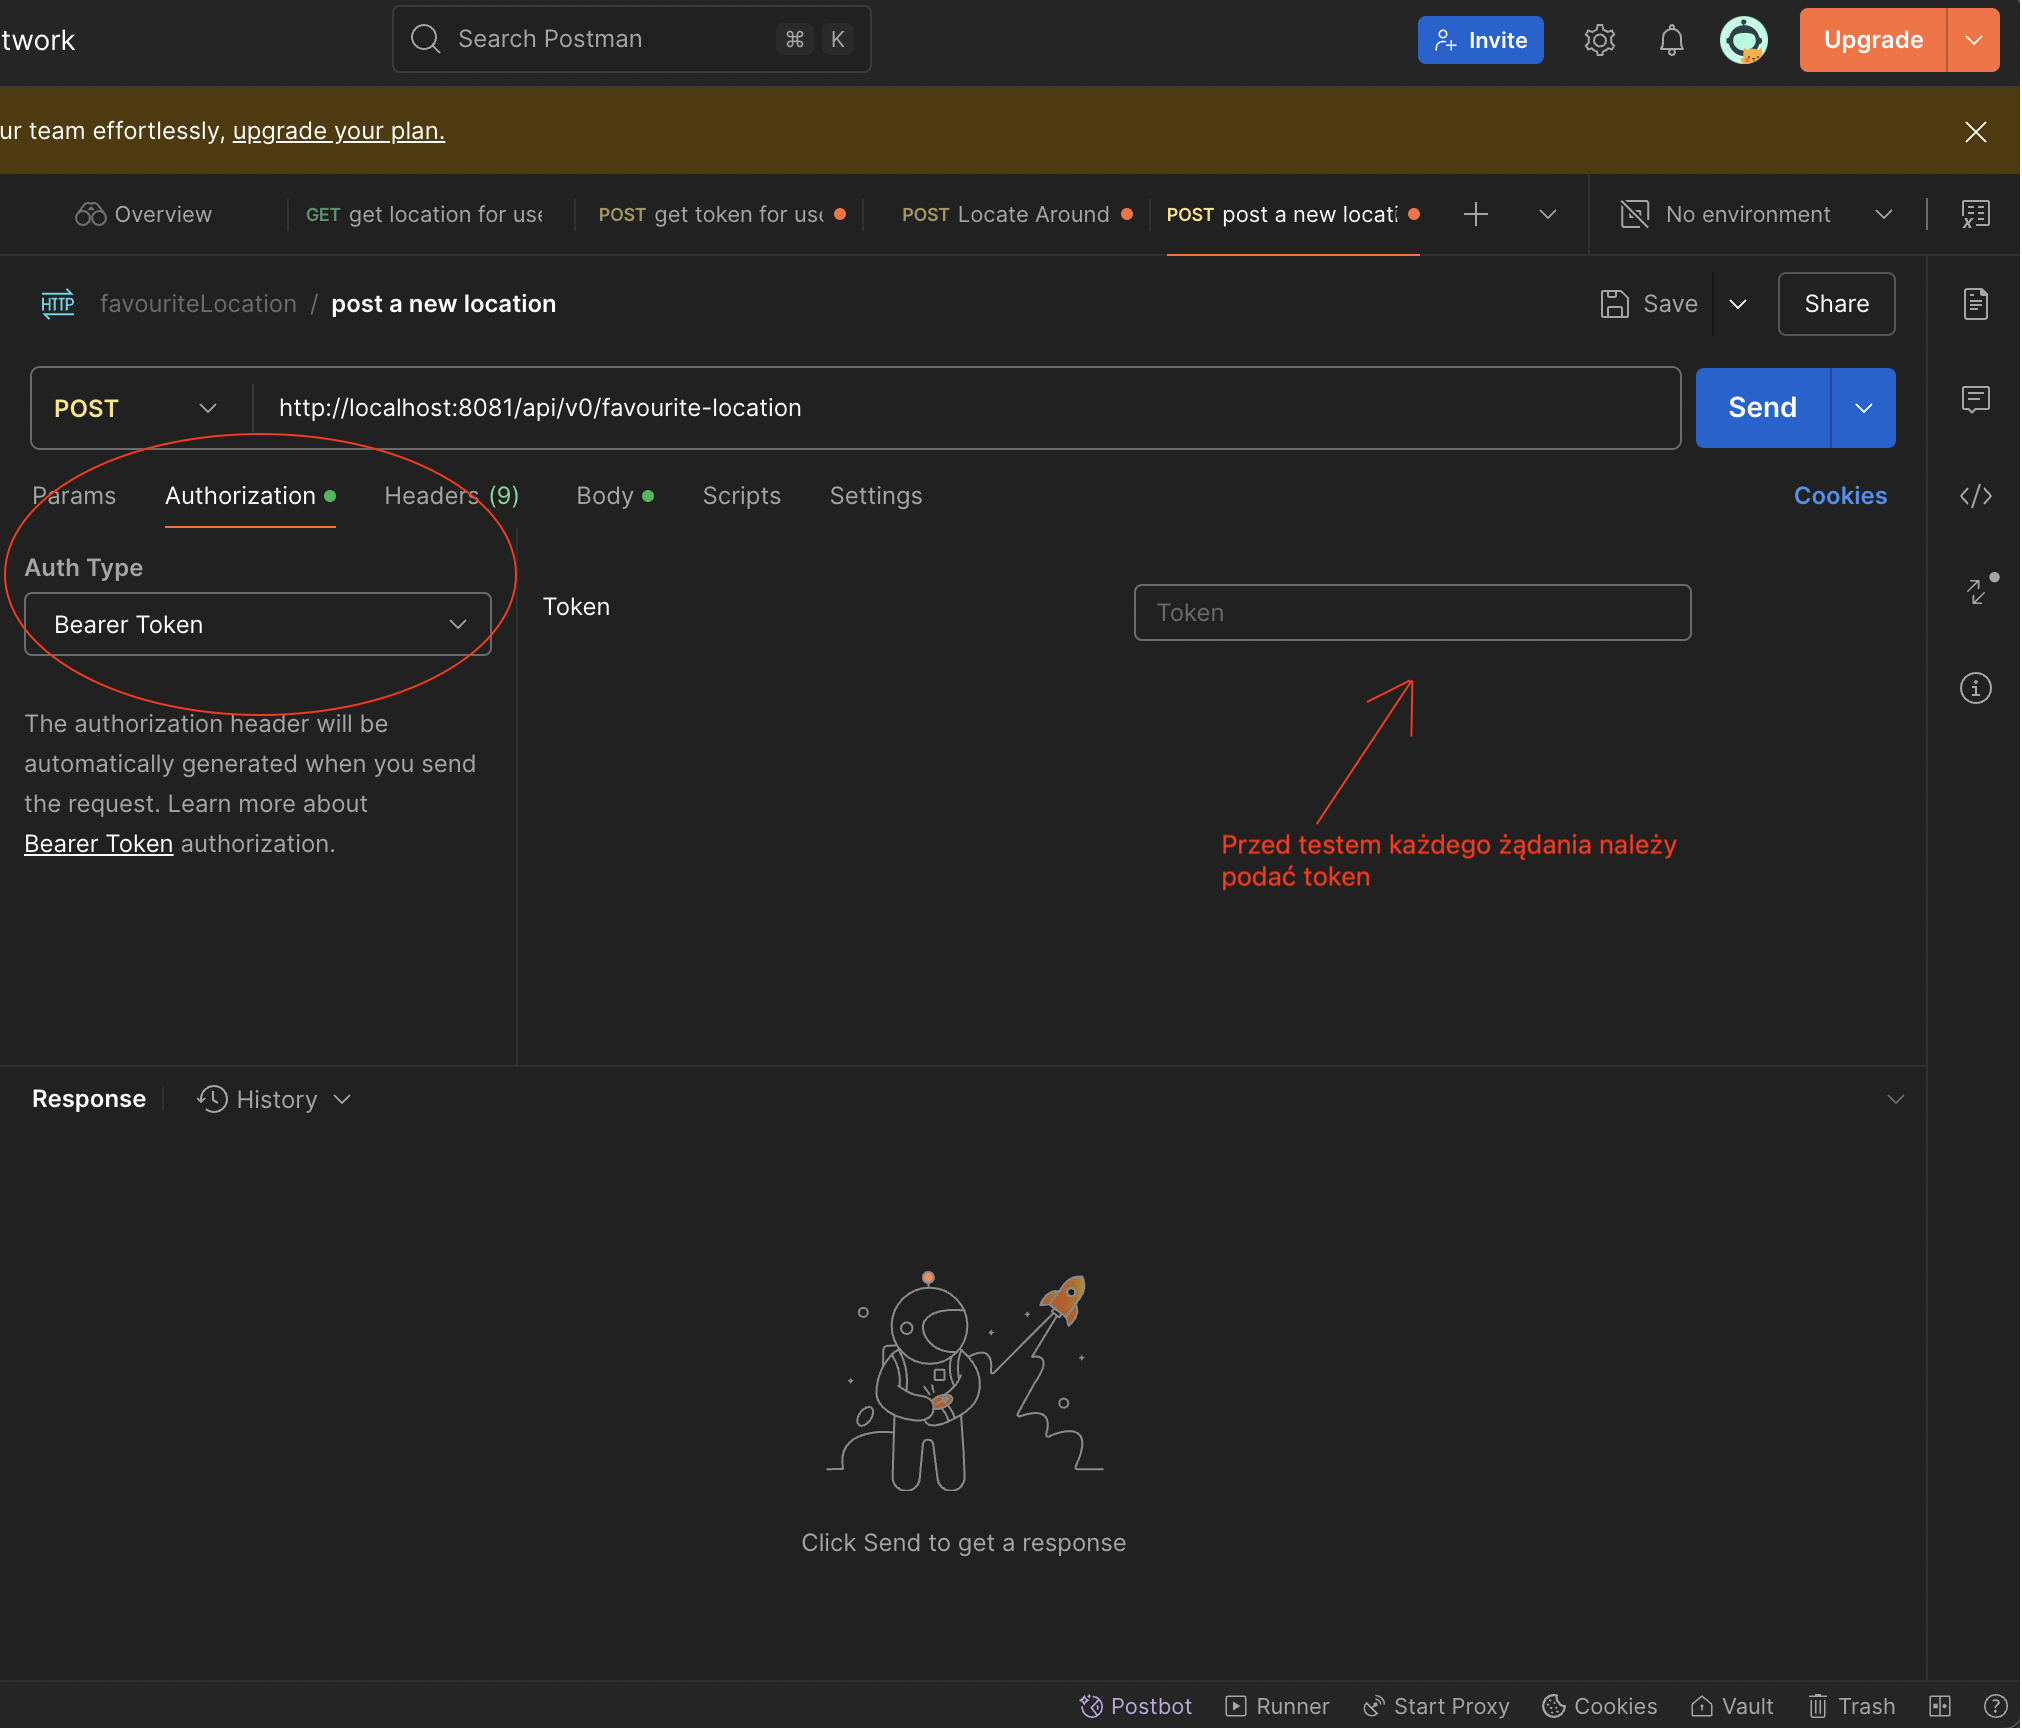
\includegraphics[width=1\linewidth]{token.png}
        \caption{testowanie endpointów z użyciem tokena JWT}
        \label{fig:enter-label}
\end{figure}

\noindent\textbf{POST /api/v0/favourite-location}
\\

\noindent
Endpoint pozwala przetestować poprawne dodanie ulubionej lokalizacji dla użytkownika oraz zapisanie jej w bazie danych. Pozwala również przetestować poprawne pobranie użytkownika z tokena JWT.

\begin{table}[h!]
\centering
\begin{tabular}{|l|l|l|}
\hline
\textbf{Parametr} & \textbf{Opis} & \textbf{Typ} \\
\hline
\texttt{score} & Ocena lokalizacji (0–100) & Integer \\
\texttt{lat} & Szerokość geograficzna & Double \\
\texttt{lon} & Długość geograficzna & Double \\
\texttt{availablePlaces} & Lista dostępnych miejsc & Array[String] \\
\texttt{notAvailablePlaces} & Lista niedostępnych miejsc & Array[String] \\
\hline
\end{tabular}
\caption{Parametry żądania POST /favourite-location}
\end{table}


\noindent\textbf{GET /api/v0/favourite-location/\{id\}}
\\

\noindent
Endpoint pozwala na pobranie z bazy danych ulubionej lokalizacji na podstawie jej identyfikatora. Sprawdzono, czy system reaguje odpowiednio, gdy szukana lokalizacja nie istnieje.Endpoint testuje również poprawność działania mechanizmu autoryzacji na podstawie tokena JWT użytkownika.
\\

\noindent\textbf{PUT /api/v0/favourite-location/\{id\}}
\\
\\
Endpoint służy do testowania funkcjonalności aktualizacji istniejącej lokalizacji na podstawie jej identyfikatora. Pozwala sprawdzić, czy system reaguje odpowiednio na próbę aktualizacji nieistniejącej lokalizacji.Endpoint testuje również poprawność działania mechanizmu autoryzacji na podstawie tokena JWT użytkownika. 

\begin{table}[h!]
\centering
\begin{tabular}{|l|l|l|}
\hline
\textbf{Parametr} & \textbf{Opis} & \textbf{Typ} \\
\hline
\texttt{score} & Ocena lokalizacji & Float \\
\texttt{lat} & Szerokość geograficzna & Double \\
\texttt{lon} & Długość geograficzna & Double \\
\texttt{availablePlaces} & Lista dostępnych miejsc & Array[String] \\
\texttt{notAvailablePlaces} & Lista niedostępnych miejsc & Array[String] \\
\hline
\end{tabular}
\caption{Parametry żądania PUT /favourite-location/\{id\}}
\end{table}

\noindent\textbf{DELETE /api/v0/favourite-location/\{id\}}
\\

\noindent
Endpoint pozwala przetestować funkcjonalność usuwania ulubionej lokalizacji z bazy danych na podstawie jej identyfikatora. Pozwala sprawdzić zachowanie systemu w przypadku usunięcia lokalizacji o identyfikatorze, który nie istnieje w bazie danych. Endpoint testuje również poprawność działania mechanizmu autoryzacji na podstawie tokena JWT użytkownika.
\\
\\
\noindent\textbf{GET /api/v0/favourite-location}

\noindent
\\
Endpoint zwracający ulubione lokalizacje wszystkich użytkowników. Pozwala sprawdzić poprawność działania mechanizmu autoryzacji na podstawie tokena JWT użytkownika.
\\

\noindent\textbf{GET /api/v0/favourite-location/user} 

\noindent
\\
Endpoint pozwalający przetestowanie funkcjonalności pobrania ulubionych lokalizacji użytkownika. Pozwala sprawdzić poprawność działania mechanizmu autoryzacji na podstawie tokena JWT użytkownika
\\

\noindent\textbf{POST /api/v0/map/locate}

\noindent
\\
Endpoint pozwala na przetestowanie{...}

\begin{table}[h!]
\centering
\begin{tabular}{|l|l|l|}
\hline
\textbf{Parametr} & \textbf{Opis} & \textbf{Typ} \\
\hline
\texttt{lat} & Szerokość geograficzna & Double \\
\texttt{lon} & Długość geograficzna & Double \\
\texttt{radius} & opis & typ \\
\texttt{types} & opis & Array[String] \\
\hline
\end{tabular}
\caption{Parametry żądania POST /map/locate}
\end{table}

\printbibliography

\end{document}
